\documentclass{beamer}

\mode<presentation>{
\usetheme{Dresden}
\setbeamercovered{transparent}
\usecolortheme{lsc}
}

\mode<handout>{
  % tema simples para ser impresso
  \usepackage[bar]{beamerthemetree}
  % Colocando um fundo cinza quando for gerar transparências para serem impressas
  % mais de uma transparência por página
  \beamertemplatesolidbackgroundcolor{black!5}
}

\usepackage{amsmath,amssymb}
\usepackage[brazil]{varioref}
\usepackage[english,brazil]{babel}
\usepackage[utf8]{inputenc}
%\usepackage[latin1]{inputenc}
\usepackage{graphicx}
\usepackage{listings}
\usepackage{url}
\usepackage{colortbl}

\beamertemplatetransparentcovereddynamic

\title[Avaliação do aprendizado dos acadêmicos da disciplina de Álgebra Linear utilizando o software AlfaGebra... \hspace{4em} \insertframenumber/\inserttotalframenumber]{Avaliação do aprendizado dos acadêmicos da disciplina de Álgebra Linear utilizando o \textit{software} AlfaGebra - módulos sistemas de equações lineares e espaço vetorial}
\author[Osmir Custódio Mariano]{%
  Osmir Custódio Mariano \\
  Orientadora: Drª. Hellena Christina Fernandes Apolinário\\
  Coorientador: Dr. Edeilson Milhomem da Silva}
  \institute[UFT]{
     Ciência da Computação\\
     Universidade Federal de Tocantins}


% Se comentar a linha abaixo, irá aparecer a data quando foi compilada a apresentação  
\date{30 de novembro de 2017}

\pgfdeclareimage[height=1cm]{inf}{img/CienciaDaComputacao.png}

% pode-se colocar o LOGO assim
\logo{\pgfuseimage{inf}}

%Gera em cada fim um novo sumário
%\AtBeginSection[]{
%  \begin{frame}<beamer>
%    \frametitle{Sumário}
%    \tableofcontents[currentsection,currentsubsection]
%  \end{frame}
%}

\begin{document}

\begin{frame}
\titlepage
\end{frame}

\begin{frame}
\frametitle[allowframebreaks]{Sumário}
\begin{small}
\tableofcontents
\end{small}
\end{frame}


\section{Introdução}
\frame{
    \frametitle{Introdução}
      \begin{itemize}
        \item Importância da Álgebra Linear;
        \begin{itemize}
            \item Disciplina de Álgebra Linear.
        \end{itemize}
	    \item Aplicação na Computação Gráfica;
	    \item Álgebra Linear no curso de Ciência da Computação na UFT.
      \end{itemize}
}

\section{Justificativa}
\frame{
    \frametitle{Justificativa}
      \begin{itemize}
        \item Ferramentas tecnológicas;
	    \item Instituições de ensino;
	    \item Dificuldade na Álgebra Linear;
	        \begin{itemize}
	            \item Pesquisas sobre dificuldade da Álgebra Linear (Celestino, 2000).
	        \end{itemize}
	    \item Ferramenta computacional para auxiliar no ensino e aprendizagem?
      \end{itemize}
}

\section{Objetivos}
\frame{
    \frametitle{Objetivo Geral}
      Desenvolver a plataforma de ensino e aprendizagem AlfaGebra e avaliar o aprendizado dos acadêmicos da disciplina de Álgebra Linear do curso de Ciência da Computação da UFT.
}

\frame{
    \frametitle{Objetivos Específicos}
        \begin{itemize}
            \item Desenvolver os módulos de sistemas de equações lineares e espaço vetorial da plataforma AlfaGebra em versão \textit{desktop} para o sistema operacional Windows;
            \item Comparar o nível de aprendizado dos acadêmicos da disciplina de Álgebra Linear com e sem a utilização do \textit{software} AlfaGebra;
        \end{itemize}
}


%\section{Conceitos propostos}
%\frame{
%    \frametitle{Conceitos propostos AlfaGebra}
%        \begin{itemize}
%            \item Computação simbólica
%            \begin{itemize}
%                \item O que é?;
%                \item Utilização para execução de operações aritméticas;
%                \item Matlab, Mathematica, etc.
%            \end{itemize}
%            \item Matlab e Álgebra Linear
%        \end{itemize}
%}

\section{Metodologia}
\frame{
    \frametitle{Pesquisa}
     \begin{itemize}
	    \item Pesquisa-ação
	    \begin{itemize}
	        \item Pesquisa em campo;
	        \item Aplicação de questionários.
	    \end{itemize}
    \end{itemize}
}
\frame{
    \frametitle{Primeiro momento da avaliação}
     \begin{itemize}
	    \item Avaliação de aprendizagem sem o uso do AlfaGebra.
	    \begin{itemize}
	        \item Aplicação de questionário.
	    \end{itemize}
    \end{itemize}
}
\frame{
    \frametitle{Desenvolvimento do \textit{software} AlfaGebra}
     \begin{itemize}
	    \item Identificação e especificação de conceitos para a plataforma;
	    \begin{itemize}
	        \item Conteúdos abordados no sistema;
	        \item Especificação de requisitos;
	        \item Prototipagem das telas.
	    \end{itemize}
	    \item Entendimento de como os conceitos são implementados;
	    \item Implementação dos conceitos da Álgebra Linear definidos;
	    \begin{itemize}
	        \item Codificação do sistema.
	    \end{itemize}
    \end{itemize}
}

\frame{
    \frametitle{Desenvolvimento do \textit{software} AlfaGebra}
     \begin{itemize}
	    \begin{figure}[htb]	
\center%6.3
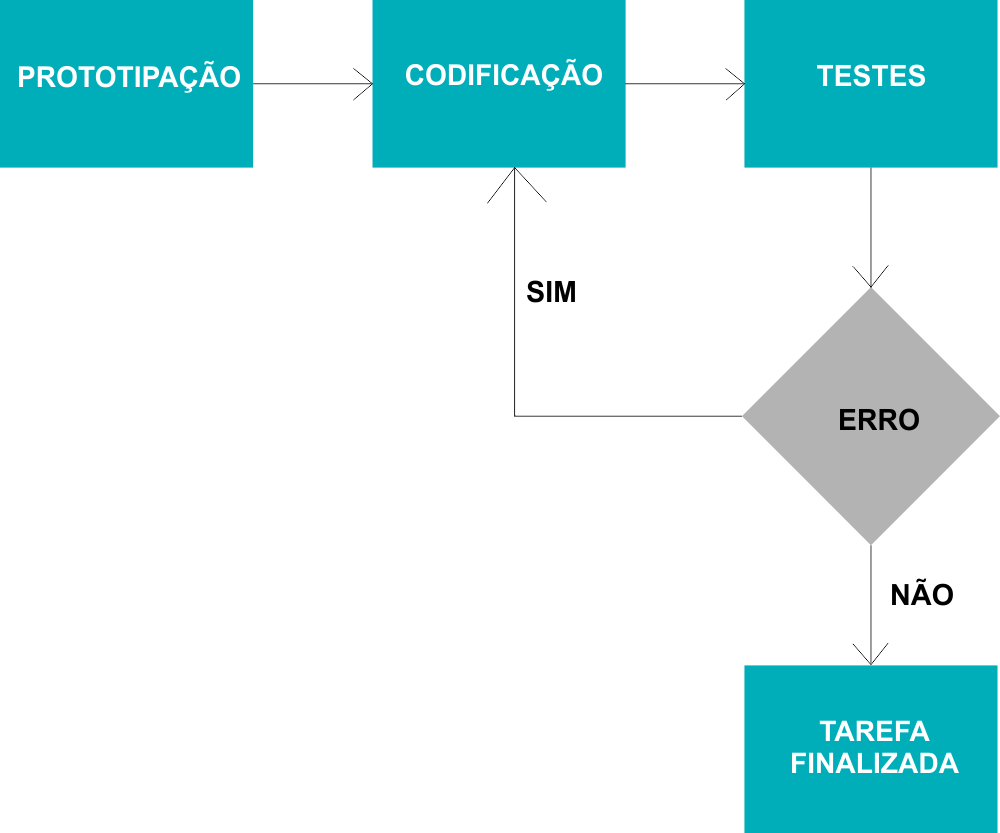
\includegraphics[width=6cm]{./img/fluxo.png}

\caption{Fluxo de desenvolvimento do \textit{software} AlfaGebra}

\end{figure}
    \end{itemize}
}
\frame{
    \frametitle{Segundo momento da avaliação}
     \begin{itemize}
	    \item Avaliação de aprendizagem com a utilização do AlfaGebra;
	    \item Análise comparativa dos resultados obtidos pelos alunos com e sem a ferramenta.
    \end{itemize}
}

\frame{
    \frametitle{Ferramentas e materiais}
        \begin{itemize}
    	    \item Java SE;
    	    \item JavaFx \textit{Sciene Builder};
    	    \item IDE Netbeans, etc.
    	    \item Metodologia de desenvolvimento ágil
    	    \begin{itemize}
    	        \item \textit{Scrum}
    	    \end{itemize}
    \end{itemize}
}

\section{Resultados preliminares}
\frame{
    \frametitle{Resultados Preliminares: primeiro momento da avaliação}
        \begin{table}[]
\centering

\begin{tabular}{|c|c|c|c|l}
\cline{1-4}
                                                       & \multicolumn{3}{c|}{\textbf{PERÍODO}}                                                &  \\ \cline{2-4}
\multirow{}{}{}                                     & \textbf{2015-2}            & \textbf{2016-1}            & \textbf{2016-2}            &  \\ \cline{1-4}
\textbf{Matriculados}                                  & 38                         & 40                         & 41                         &  \\ \cline{1-4}
\cellcolor[HTML]{67FD9A}\textbf{Aprovados}             & \cellcolor[HTML]{67FD9A}10 & \cellcolor[HTML]{67FD9A}20 & \cellcolor[HTML]{67FD9A}15 &  \\ \cline{1-4}
\cellcolor[HTML]{EFEFEF}\textbf{Reprovados por faltas} & \cellcolor[HTML]{EFEFEF}21 & \cellcolor[HTML]{EFEFEF}12 & \cellcolor[HTML]{EFEFEF}23 &  \\ \cline{1-4}
\cellcolor[HTML]{FD6864}\textbf{Reprovados por notas}  & \cellcolor[HTML]{FD6864}7  & \cellcolor[HTML]{FD6864}8  & \cellcolor[HTML]{FD6864}3  &  \\ \cline{1-4}
\end{tabular}
\caption{Dados dos quantitativos de alunos nos três últimos semestres, referentes a aprovados por notas, reprovados por faltas e reprovados por notas}
\label{dados_alunos_3_ultimos_semestres}
\end{table}
        \begin{itemize}
    	    \item 51,37\% de evasões
        \end{itemize}
}
\frame[allowframebreaks]{
    \frametitle{Coleta de dados}
        \begin{itemize}
    	    \item Grau de dificuldade da disciplina de Álgebra Linear;
    	    \begin{figure}[htb]	
\center%6.3
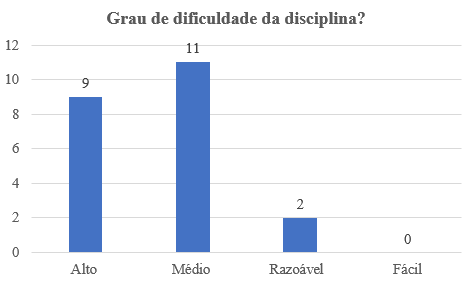
\includegraphics[width=6cm]{./img/grau_dificuldade.png}

\caption{Grau de dificuldade dos alunos}

\end{figure}
            \item 40,90\% alto, 50\% médio e 9,10\% razoável.
            
            \item Frequência procuram o professor para sanar dúvidas;
            \begin{figure}[htb]	
\center%6.3
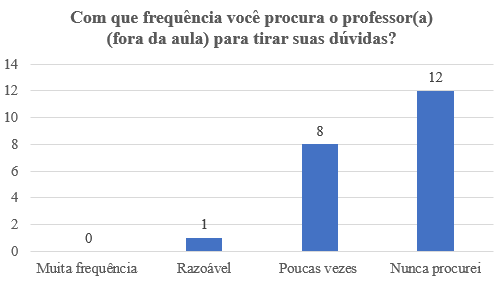
\includegraphics[width=7cm]{./img/frequencia_professor.png}

\caption{Frequência em que os alunos procuram o professor}

\end{figure}


            \item 4,54\% frequente, 36,36\% às vezes e 54,54\% nunca.
            
            \item Utilização de tecnologia para estudo
            \begin{figure}[htb]	
\center%6.3
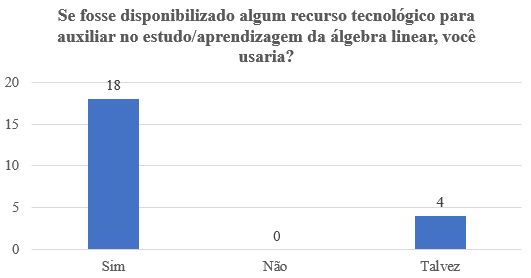
\includegraphics[width=7cm]{./img/tecnologia_usa.png}

\caption{Utilização de tecnologia para o estudo}

\end{figure}     
            \item 81,81\% usariam e 18,10\% indecisos.
        \end{itemize}
}



\section{Conclusões}
\frame{
    \frametitle{Conclusões}
        \begin{itemize}
    	    \item Dificuldade da disciplina de Álgebra Linear;
    	    \item Recursos tecnológicos para o ensino e aprendizagem;
    	    \item Contribuição AlfaGebra.
        \end{itemize}
}

\frame{
    \frametitle{Continuação do trabalho}
        \begin{itemize}
    	    \item Conclusão do desenvolvimento do \textit{software} AlfaGebra;
    	    \item Disponibilidade do \textit{software};
    	    \item Aplicação de questionários;
    	    \item Identificar na melhora do aprendizado com o AlfaGebra;
    	    \item Análise dos resultados.
        \end{itemize}
}


\section{Referências}
\frame[allowframebreaks]{
    \frametitle{Referências}
  
    \bibliographystyle{sbc}%apalike
    \bibliography{tcc1}
    
    \nocite{2011:Furtado}
    \nocite{2000:lima}
    \nocite{2000:celestino}
   
}





\begin{frame}
\titlepage
\end{frame}

\end{document}